\documentclass[border=4pt]{standalone}
\usepackage[fontset=fandol]{ctex}
\usepackage{amsmath,amssymb,bm,tikz}
\usetikzlibrary{arrows.meta,calc,decorations.pathmorphing}
\pagestyle{empty}
\begin{document}

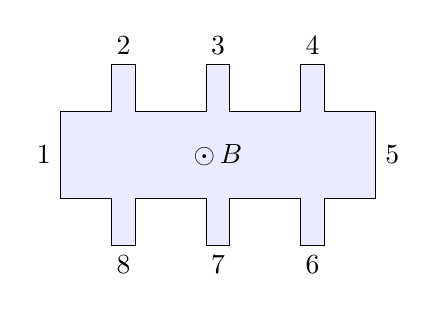
\begin{tikzpicture}
\draw[fill=blue!8](-2,-.55)--(-1.35,-.55)--(-1.35,-1.15)--(-1.05,-1.15)--(-1.05,-.55)--(-.15,-.55)--(-.15,-1.15)--(.15,-1.15)--(.15,-.55)--(1.05,-.55)--(1.05,-1.15)--(1.35,-1.15)--(1.35,-.55)--(2,-.55)--(2,.55)--(1.35,.55)--(1.35,1.15)--(1.05,1.15)--(1.05,.55)--(.15,.55)--(.15,1.15)--(-.15,1.15)--(-.15,.55)--(-1.05,.55)--(-1.05,1.15)--(-1.35,1.15)--(-1.35,.55)--(-2,.55)--cycle;
\node[left]at(-2,0){1};\node[right]at(2,0){5};
\foreach \x/\n in {-1.2/2,0/3,1.2/4}\node[above]at(\x,1.15){\n};
\foreach \x/\n in {-1.2/8,0/7,1.2/6}\node[below]at(\x,-1.15){\n};
\node at(0,0){$\odot\,B$};
\end{tikzpicture}

\end{document}
